\documentclass{letask}

\begin{document}
\begin{titlepage}
\center % Center everything on the page
 
%----------------------------------------------------------------------------------------
%	HEADING SECTIONS
%----------------------------------------------------------------------------------------

\textsc{\LARGE Московский\\[-0.2cm]Физико-Технический Институт\\[0.1cm]\large (государственный университет)}\\[1.5cm] % Name of your university/college
\textsc{\Large Кафедра общей физики}\\[0.1cm] % Major heading such as course name
\textsc{\large Лабораторная работа \textnumero  4.4.1}\\[0.5cm] % Minor heading such as course title

%----------------------------------------------------------------------------------------
%	TITLE SECTION
%----------------------------------------------------------------------------------------

\HRule
\\[0.4cm]
{ \huge \bfseries Амплитудная\\[0.2cm]
дифракционная решетка}
\\[0.6cm] % Title of your document
\HRule
\\[1.5cm]


 
%----------------------------------------------------------------------------------------
%	AUTHOR SECTION
%----------------------------------------------------------------------------------------

\begin{minipage}{0.4\textwidth}
	\begin{flushleft} \large
		\textsf{Студент}
		
		Ришат \textsc{Исхаков} \\[-0.15cm]
		513 группа
	\end{flushleft}
\end{minipage}
~
\begin{minipage}{0.4\textwidth}
	\begin{flushright} \large
		\textsf{Преподаватель}
		
		Александр Александрович \\[-0.15cm]
		\textsc{Казимиров} % Supervisor's Name
	\end{flushright}
\end{minipage}

\begin{bottompar}
	\begin{center}
		
\includegraphics[width = 80 mm]{logo.jpg}
	\end{center}
	{\large \today}

\end{bottompar}
\vfill % Fill the rest of the page with whitespace

\end{titlepage}

\textbf{Цель работы:}
изучение интерферометра Фабри-Перо и определение его характеристик, как спектрального прибора.
\textbf{В работе используются:} интерферометры Фабри-Перо, линзы, светофильтр, ртутная лампа ПРК-2, высокочастотная натриевая лампа, катетометры КМ-6.

\section{Теоретическая часть}

\subsection*{Интерферометр Фабри-Перо}

\begin{wrapfigure}[10]{r}{8.5 cm}
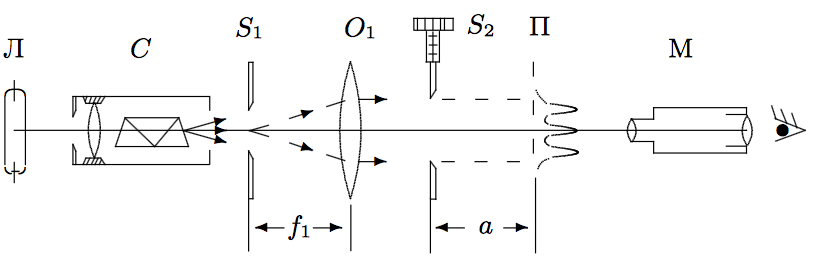
\includegraphics[width = 8 cm]{img1}
\caption{Интерферометр Фабри-Перо}
\end{wrapfigure}

Интерферометр Фабри-Перо состоит из двух отражающих пластин, внутренние поверхности которых хорошо отполированы и установлены параллельно друг другу. Его можно рассматривать как плоскопараллельную воздушную пластину, на которой происходят многократные отражения и интерференция световых лучей. Интерференционная картина, наблюдаемая в фокальной плоскости линзы Л, состоит из концентрических колец. 
Для двух соседних лучей, распространяющихся между зеркалами интерферометра под углом $\theta$, разность хода определяется соотношением
 
\begin{equation}
\Delta = 2 L \cos \theta,
\label{eq:dif}
\end{equation}

где $L$~--~расстояние между зеркалами интерферометра.
Будем считать, что поглощение света в зеркалах отсутствует, что достигается лишь при целых значениях отношения $\Delta / \lambda$.

Интерференционная картина состоит из узких светлых колец, разделенных широкими промежутками, расстояния между которыми мы будем измерять.

\subsection*{Измерение длин волн $\lambda$ и расстояний $d \lambda$ между спектральными линиями.}

Исследуем диаметры интерференционных колец, предполагая, что угол $\theta$ достаточно мал.
Рассмотрим два кольца с разным порядком интерференции: $m_i$ и $m_j$ соответственно. 
Из~(\ref{eq:dif}) и условия отсутствия поглощения следует, что светлое кольцо порядка $m$ образуется при 

\begin{equation}
\label{eq:m}
\Delta = 2 L \cos \theta = m \lambda \; (m - \text{целое}).
\end{equation}

При уменьшении угла $\theta$ порядок интерференции возрастает, то есть больший порядок соответствует кольцам меньшего диаметра.

Для малых углов $\theta$:

\begin{equation}
2L \left( 1 - \dfrac{\theta_i^2}{2} \right) = m_i \lambda; \quad
2L \left( 1 - \dfrac{\theta_j^2}{2} \right) = m_j \lambda.
\end{equation}

Вычтем второе уравнение из первого и рассмотрим два соседних кольца:

\[
L(\theta_j^2-\theta_i^2) = (j - i) \lambda
\]

Диаметр $D$ кольца в фокальной плоскости линзы связан с ее фокусным расстоянием:

\[
D = 2 f \theta
\]

Тогда выразим $\lambda$ из уравнения:

\begin{equation}
\lambda = \dfrac{L}{4 f^2} \dfrac{D_j^2 - D_i^2}{j-i}
\end{equation}

Пусть в интерферометре Фабри-Перо наблюдается система колец для двух близких спектральных линий $\lambda$ и $\lambda + d\lambda$, дифференцируя (\ref{eq:m}) при малых $\theta$ найдем 

\[
-2L \theta d \theta = m d \lambda,
\] откуда следует:

\begin{equation}
d \lambda = - \dfrac{2 L \theta}{m} \simeq - \lambda \theta d \theta = - \dfrac{\lambda \overline{D}}{4 f^2} dD,
\label{eq:dlambda}
\end{equation}
где $\overline{D}$ ~---~ средний диаметр колец, а $dD$~---~ разность диаметров колец, образующихся для спектральных линий с длинами волна $\lambda$, и $\lambda + d\lambda$ при одинаковом порядке интерференции. С помощью формулы (\ref{eq:dlambda}) можно определять $d \lambda$, не зная постоянной интерферометра $L$.

\subsection*{Дисперсия интерферометра}

Отношение $D^* = dl /d\lambda,$ где $dl$~--~ расстояние между спектральными линиями в плоскости спектра, а $d\lambda$~--~разность длин волн этих линий, называют \textsc{линейной дисперсией} спектрального прибора. Линейная дисперсия для интерферометра Фабри-Перо выражается через угловую $(d \Theta / d \lambda)$ (формула (\ref{eq:dlambda}):

\[
D^* = f \dfrac{d \Theta}{d \lambda} = \dfrac{dD}{2 d \lambda} = \dfrac{2 f^2}{\lambda D}
\]

\subsection*{Дисперсионная область}

Областью дисперсии называют максимальный интервал длин волн $\Delta \lambda$, при котором еще не происходит перекрытия интерференционных полос соседних порядков. Пусть накладывается кольцо $(m+1)\text{-го порядка}$ для длины волны $\lambda$ и кольца $m\text{-го порядка}$ для длины волны $\lambda + \Delta \lambda$:

\begin{equation}
m(\lambda + \Delta \lambda) = (m+1)\lambda,
\end{equation}
откуда 

\begin{equation}
\Delta \lambda = \dfrac{\lambda}{m} \approx \dfrac{\lambda^2}{2L}
\end{equation}

\subsection*{Разрешающая способность интерферометра Фабри-Перо}

Разрешающая способность спектрального прибора определяется соотношением:

\begin{equation}
R = \dfrac{\lambda}{\delta \lambda},
\end{equation}

где $\delta \lambda$~--~минимальная разность длин волн, разрешимая прибором вблизи волны $\lambda$. Если определить ширину линии на уровне, на котором интенсивность падает в два раза по сравнению с максимальным значением в середине линии, можно из критерия разрешения Релея определить разрешающую способность:

\begin{equation}
R \approx \dfrac{2 \pi L \sqrt{r}}{\lambda (1-r)}
\end{equation}

\section{Установка и параметры измерения}

\begin{wrapfigure}[14]{l}{13 cm}
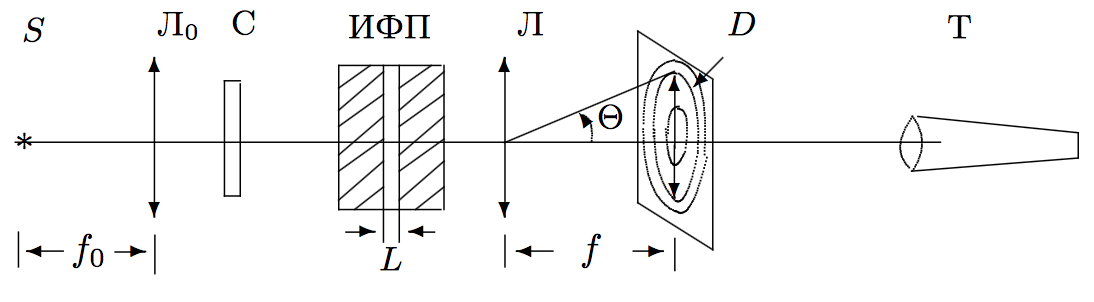
\includegraphics[width =  \lw]{plan}
\caption{Схема экспериментальной установки}
\end{wrapfigure}

$$f_1 = 110 \quad \mm$$
$$f_2 = 94 \quad \mm$$
$$L(Hg) \simeq 0.1 \quad \mm$$
$$L(Na) \simeq 3 \quad \mm $$
\vspace{1 cm}


Свет от лампы $S$, пройдя через линзу $\text{Л}_0$ светофильтр $C$ попадает в интерферометр Фабри-Перо (ИФП). Линза $\text{Л}_0$ формирует пучек лучей. Интерференционные кольца наблюдаются в фокальной плоскости линзы Л.

\subsection*{Ртутная лампа}

Сначала измерим координаты $i-\text{ых}$ колец, двигаясь снизу вверх. По ним можно определить диаметр каждого кольца.

\begin{table}[H]
\centering
\begin{tabular}{|c|c|c|c|c|c|c|}
\hline
i            & 1      & 2      & 3      & 4      & 5       & 6       \\ \hline
$x_{\text{н}}, \mm$ & 166.61 & 172.33 & 175.52 & 177.99 & 179.85  & 181.87  \\ \hline
$x_{\text{в}}, \mm$ & 155.53 & 152.38 & 149.92 & 147.88 & 146.12  & 144.48  \\ \hline
$D, \mm$     & 11.08  & 19.95  & 25.6   & 30.11  & 33.73   & 37.39   \\ \hline
$D^2, \mm^2$ & 122.77 & 398.00 & 655.36 & 906.61 & 1137.71 & 1398.01 \\ \hline
\end{tabular}
\caption{Измерение диаметров зеленых колец}
\end{table}

Оценим максимальный порядок интерференции $m$ (номер центрального кольца) для желтой и зеленой линии ртути:

\[
m_\text{зел} = \dfrac{2L \cos \theta}{\lambda} \approx \dfrac{2L}{\lambda} = 357; \qquad m_\text{жел} = 345
\]

Оценим дисперсионную область:

\[ \Delta \lambda = \dfrac{\lambda}{m} \]
\[ \lambda_\text{ж} = 160 \; \angstrom; \qquad \lambda_\text{з} = 170 \; \angstrom \]

Построим график зависимости $D^2_i = f(i)$

\begin{figure}[H]
\centering
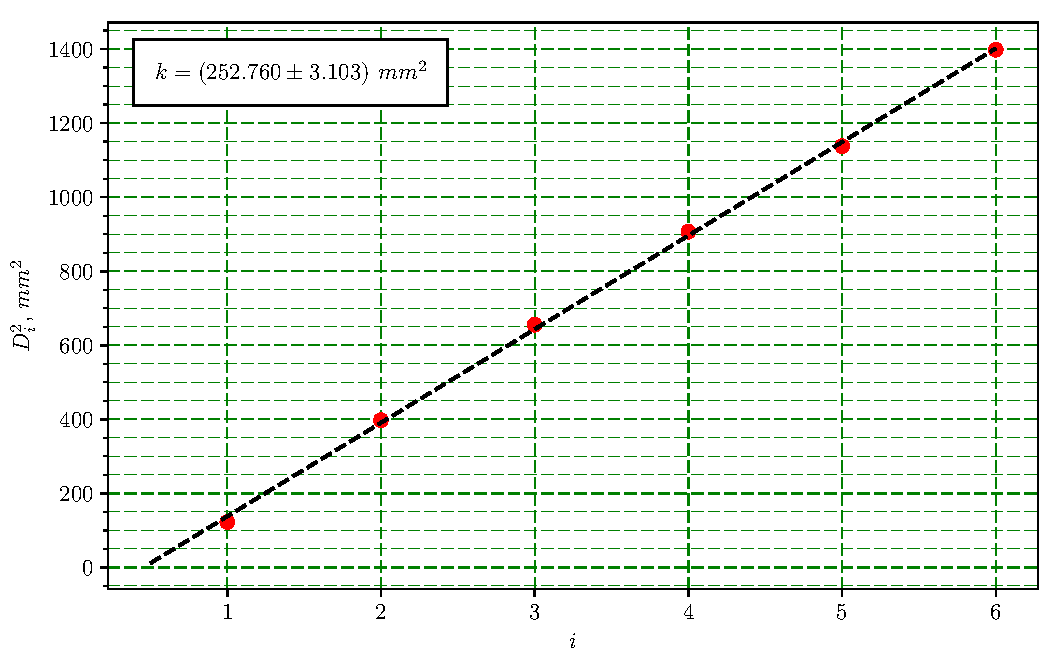
\includegraphics[width = 0.85 \lw]{graph1}
\caption{График зависимости $D^2_i = f(i)$ для зеленых колец ртути}
\end{figure}

Определим постоянную интерферометра $L$ (расстояние между зеркалами) по формуле (\ref{eq:dlambda}), учитывая, что $\lambda = 5461 \angstrom$

\[
L = \dfrac{4f^2 \lambda}{k} = (1.04 \pm 0.09) \cdot 10^{-4} \; \m
\]

\begin{table}[H]
\centering
\begin{tabular}{|c|c|c|c|c|c|c|}
\hline
i                 & 1           & 2           & 3           & 4           & 5           & 6           \\ \hline
$x_{\text{н1}}, \mm$     & 166.78      & 172.53      & 175.64      & 178.13      & 180.28      & 182.15      \\ \hline
$x_{\text{в1}}, \mm$     & 160.85      & 155.22      & 151.99      & 149.47      & 147.19      & 145.42      \\ \hline
$x_{\text{н2}}, \mm$     & 169.53      & 173.65      & 176.61      & 178.84      & 181.1       & 182.74      \\ \hline
$x_{\text{в2}}, \mm$     & 158.32      & 153.98      & 151.27      & 148.74      & 146.71      & 144.88      \\ \hline
$D_1, \mm$        & 5.93        & 17.31       & 23.65       & 28.66       & 33.09       & 36.73       \\ \hline
$D_2, \mm$        & 11.21       & 19.67       & 25.34       & 30.1        & 34.39       & 37.86       \\ \hline
$\overline{D}, \mm$          & 8.57        & 18.49       & 24.50       & 33.74       & 33.56       & 37.30       \\ \hline
$\Delta D, \mm$   & 5.28        & 2.36        & 1.69        & 1.44        & 1.3        & 1.13        \\ \hline
$1/\Delta D, \mm$ & 0.19 & 0.42 & 0.59 & 0.69 & 0.77 & 0.88 \\ \hline
\end{tabular}
\caption{Измерение диаметров желтых колец}
\end{table}

Построим график $\overline{D}(1/\Delta D)$ для желтых колец ртути.

\begin{figure}[H]
\centering
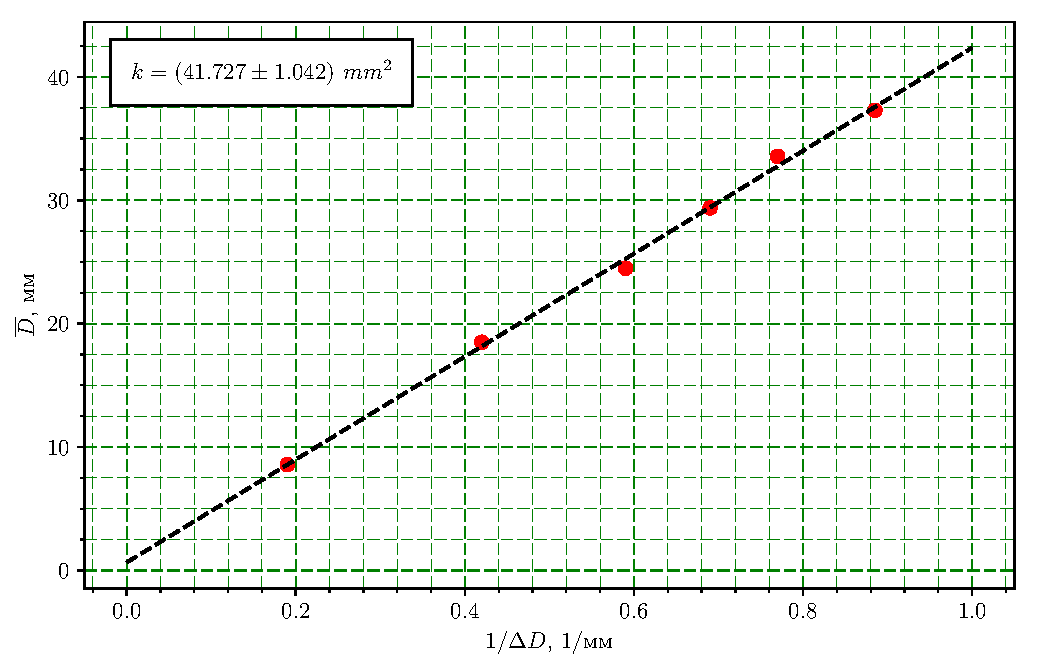
\includegraphics[width = 0.85 \lw]{graph2}
\caption{График зависимости $\overline{D}(1/\Delta D)$ для желтых колец ртути}
\end{figure}

По углу наклона прямой рассчитаем разность длин волн для желтой пары линий ртути:

\[ \Delta \lambda = \dfrac{\lambda \overline{D} \Delta D}{4 f^2} = \dfrac{\lambda k}{4f^2} = (4.9 \pm 0.3) \; \angstrom \]

Измерим ширину кольца:
\[ \delta r = (0.8 \pm 0.01) \;  \mm \]

Оценим аппаратную разрешающую способность:
\[ R = \dfrac{\lambda}{\delta \lambda} = \dfrac{4f^2}{D \delta r} = 5040 \pm 20 \]

Найдем теоретическое значение добротности для $r = 0.85$:
\[ Q = \dfrac{2 \pi L}{\lambda (1 - r)} = 7600 \]

Найдем число интерферирующих лучей: 
\[N = \dfrac{Q}{m} = 21\]


\subsection*{Натриевая лампа}

\begin{table}[H]
\centering
\begin{tabular}{|c|c|c|c|c|c|c|}
\hline
i                 & 1      & 2      & 3      & 4      & 5      & 6      \\ \hline
$x_{\text{н1}}, \mm$     & 165.76 & 169.92 & 172.64 & 174.54 & 176.52 & 178.23 \\ \hline
$x_{\text{в1}}, \mm$     & 155.56 & 151.69 & 148.95 & 146.77 & 144.9  & 143.19 \\ \hline
$x_{\text{н2}}, \mm$     & 167.39 & 170.85 & 173.46 & 175.28 & 177.09 & 178.74 \\ \hline
$x_{\text{в2}}, \mm$     & 154.07 & 150.73 & 148.23 & 146.17 & 144.32 & 142.66 \\ \hline
$D_1, \mm$        & 10.2   & 18.23  & 23.69  & 27.77  & 31.62  & 35.04  \\ \hline
$D_2, \mm$        & 13.32  & 20.12  & 25.23  & 29.11  & 32.77  & 36.08  \\ \hline
$D, \mm$          & 11.76  & 19.18  & 24.46  & 28.44  & 32.20  & 35.56  \\ \hline
$D^2, \mm$	  & 138.30	 & 367.68	&598.29	&808.83	&1036.52	&1264.51 \\ \hline
$\Delta D, \mm$   & 3.12   & 1.89   & 1.54   & 1.34   & 1.15   & 1.04   \\ \hline
$1/\Delta D, \mm$ & 0.32   & 0.53   & 0.65   & 0.75   & 0.87   & 0.96   \\ \hline
\end{tabular}
\caption{Измерение диаметров желтых колец натрия}
\end{table}

Построим график зависимости $D^2_i = f(i)$

\begin{figure}[H]
\centering
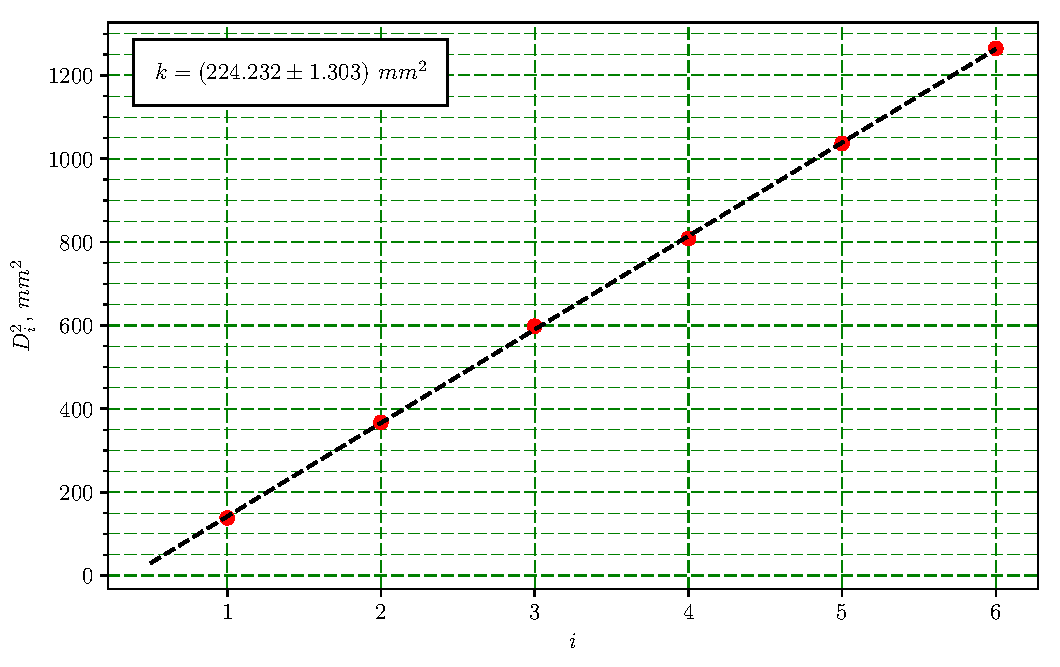
\includegraphics[width = 0.85 \lw]{graph3}
\caption{График зависимости $D^2_i = f(i)$ для зеленых колец натрия}
\end{figure}

Определим постоянную интерферометра $L$ (расстояние между зеркалами) по формуле (\ref{eq:dlambda}), учитывая, что $\lambda = 5893 \angstrom$

\[
L = \dfrac{4f^2 \lambda}{k} = (0.92 \pm 0.06) \cdot 10^{-4} \; \m
\]

Построим график $\overline{D}(1/\Delta D)$ для колец натрия.

\begin{figure}[H]
\centering
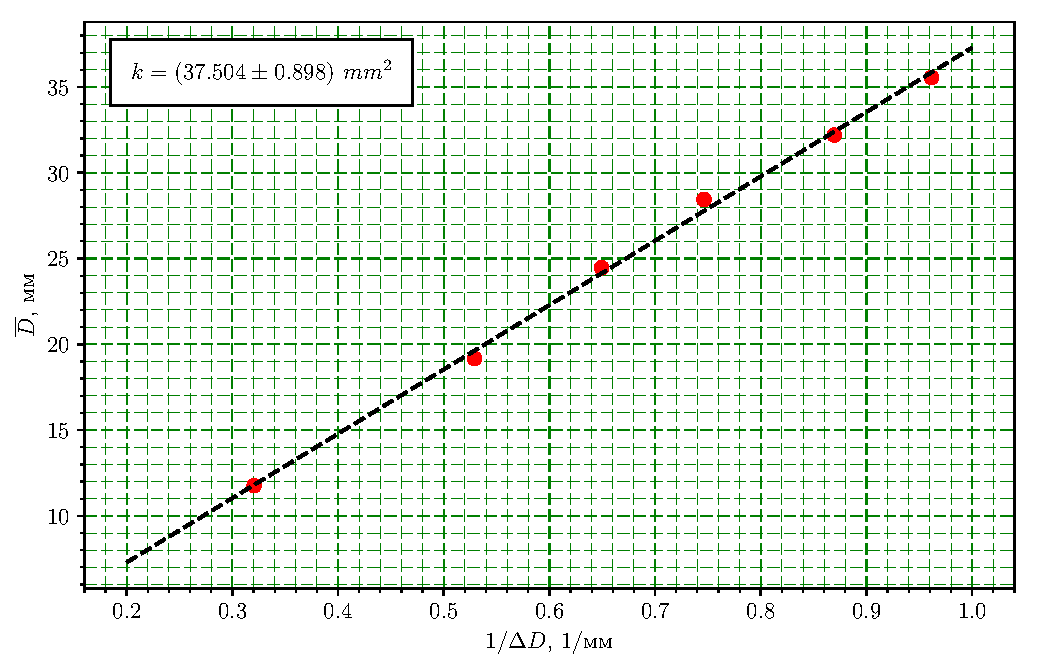
\includegraphics[width = 0.85 \lw]{graph4}
\caption{График зависимости $\overline{D}(1/\Delta D)$ для колец натрия}
\end{figure}

По углу наклона прямой рассчитаем разность длин волн для желтой пары линий натрия:

\[ \Delta \lambda = \dfrac{\lambda \overline{D} \Delta D}{4 f^2} = \dfrac{\lambda k}{4f^2} = (6.3 \pm 0.2) \; \angstrom
\]
 
Оценим экспериментальные и теоретические значения линейной дисперсии интерферометров:

\[ D^*_\text{эксп} = \dfrac{\Delta D}{2 \Delta \lambda}; \quad  D^*_\text{теор} = \dfrac{2f^2}{\lambda D} \]

\begin{table}[H]
\centering
\begin{tabular}{|c|c|c|c|}
\hline
$D^*_\text{эксп}, \; \mm/\angstrom$ & $D^*_\text{теор}, \; \mm/\angstrom$ & $\sigma D^*_\text{эксп}, \; \mm/\angstrom$ &                         \\ \hline
0.54              & 0.44              & 0.08                     & \parbox[h]{8 pt}{\multirow{6}{*}{\rotatebox[origin=c]{90}{ртуть}}}  \\ \cline{1-3}
0.24              & 0.25              & 0.04                     &                         \\ \cline{1-3}
0.17              & 0.19              & 0.03                     &                         \\ \cline{1-3}
0.15              & 0.16              & 0.02                     &                         \\ \cline{1-3}
0.13              & 0.14              & 0.02                     &                         \\ \cline{1-3}
0.12              & 0.13              & 0.02                     &                         \\ \hline
0.25              & 0.24              & 0.03                     & \parbox[h]{10 pt}{\multirow{6}{*}{\rotatebox[origin=c]{90}{натрий}}} \\ \cline{1-3}
0.15              & 0.15              & 0.02                     &                         \\ \cline{1-3}
0.12              & 0.11              & 0.02                     &                         \\ \cline{1-3}
0.11              & 0.10              & 0.01                     &                         \\ \cline{1-3}
0.09              & 0.09              & 0.01                     &                         \\ \cline{1-3}
0.08              & 0.08              & 0.01                     &                         \\ \hline
\end{tabular}
\caption{Экспериментальные и теоретические значения линейной дисперсии}
\end{table}

Измерим ширину кольца:
\[ \delta r =  (0.52 \pm 0.01) \; \mm \]
Оценим аппаратную разрешающую способность:
\[ R = \dfrac{\lambda}{\delta \lambda} = \dfrac{4f^2}{D \delta r} = 4930 \pm 20 \]
Найдем теоретическое значение добротности для $r = 0.85$:
\[ Q = \dfrac{2 \pi L}{\lambda (1 - r)} = 7100 \]
  
Найдем число интерферирующих лучей: 
\[N = \dfrac{Q}{m} = 20\]


\section{Вывод}

Мы изучили работу интерферометр Фабри-Перо, определили его постоянную, аппаратную разрешающую способность, значение линейной дисперсии. Полученные результаты с точностью до погрешности совпадают с теоретическими/заводскими значениями.

\end{document}
